\scanpage{4}

% ll. 1–2
\mspage{2}
\[
\begin{aligned}
\text{Considérons}\quad A_x&=E(x)\cap\deleted{\unsure{S}}\{S^*-\sigma_t(x)\}=E(x)\cap(E(v)^*\cup E(w)^*)\\
&=E(x)-\{u,\sigma(x)\}
\end{aligned}
\]

% ll. 3–8
son cardinal est $10-2=8$ par b), \deleted{supposons que} : il se décompose en réunion disjointe de $E(\deleted{\unsure{y}}x)\cap E(v)^*=A_{\unsure{u|v}}$ et $E(x)\cap E(w)^*=A_w$, supposons que l'un \deleted{des deux soit} \deleted{\unsure{$A_v$ soit (dans limite)|$A_v,A_w$ (disons $A_w$)}} de cardinal $\ne4$, p. ex. $>4$ (sinon on intervertit $v$ et $w$). Alors $\exists\,y,y'$ liés dans $E(v)^*$ qui sont liés \unsure{au|à un} $=$ $x$, absurde on a vu.

% ll. 9–10
\uline{Corollaire} Si $x\in E(u)$, $y\in E(v)$ sont liés, $\sigma_{\unsure{t|T}}(x)$ et $\sigma(y)$ sont liés (et inv.)

% ll. 11–12
Si $x$ lié à $y$, $x$ non lié à $\inserted{y'=}\sigma_t(y)$, donc $\sigma_t(x)$ lié à $y'$, cqfd.

% l. 13
\uline{Corollaire} $\sigma_T=\sigma$ est un autom. de $S$.

% left beside cancelled lemma
\margin{\uline{NB}}

% ll. 14–18, crossed block
\deleted{\uline{Lemme 4} Soient $x,y\in E(u)^*$ non liés. Alors
\[
\begin{aligned}
&\operatorname{Card} E(x)\cap E(y)\cap E(v)^*=2.\\
&\text{i.e.}\quad \operatorname{card} w_x
\end{aligned}
\]
\uline{Dém} S'il était $\ne2$, on peut supposer qu'il est $>2$ [ quitte à remplacer \unsure{$x$|$y$} par $\sigma(y)$}

% left of cancelled proof
\figure{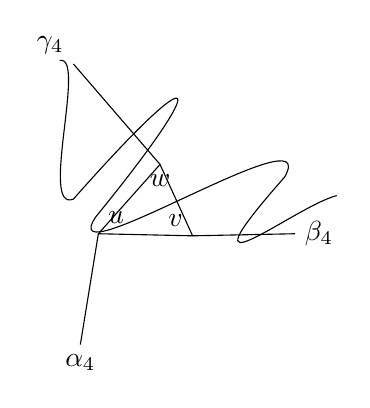
\begin{tikzpicture}[scale=.88]
\draw (0,-1.6) node[below] {$\alpha_4$} -- (.26,0) -- (1.15,1) -- (1.62,-.03) -- (.26,0);
\draw (1.15,1) -- (-.1,2.45) node[above left] {$\unsure{\gamma_4}$};
\draw (1.62,-.03) -- (3.1,0) node[right] {$\beta_4$};
\node[above right] at (.26,0) {$u$}; \node[above left] at (1.62,-.03) {$v$}; \node[below] at (1.15,1) {$w$};
\draw[thin] (-.3,2.5) .. controls (.1,2.6) and (-.6,.3) .. (-.1,.5) .. controls (1.8,2.65) and (1.9,2.3) .. (.22,.24) .. controls (-.4,-.7) and (3.5,1.8) .. (2.95,.82) .. controls (1.3,-1.05) and (3.1,.4) .. (3.7,.55);
\end{tikzpicture}}

% right of crossed block
\margin{\unsure{Introduire|Int. décrire|Introduisons} $P_u=E(u)^*/\sigma$ etc et $w_v(x)=\text{image de } E(x)\cap E(v)^*$ dans $P_v$, avec $w_v(\sigma x)=\unsure{\complement|C}w_v(x)$.}

% ll. 19–20
Soient $x,y\in\deleted{\unsure{S^*}}E(u)$, considérons

% ll. 19–20 right
\[
\begin{aligned}
w_v(x)&=E(x)\cap E(v)^*\\
w_v(y)&=E(y)\cap E(v)^*
\end{aligned}
\]

% ll. 21–23
\deleted{et une} \deleted{donc} on peut considérer $w_v(y)$ et $w_v(x)$ comme 2 sections de $E(v)^*$ sur $P_v=E(v)^*/\mathbb F_2$, donc leur différence est un élmt \deleted{\illegible{1}}.

% l. 24
\[
\delta_v(x,y)\in\mathbb F_2(P_v)
\]

% right of l. 24
\margin{\uline{NB} $\delta_v(x,\sigma(y))=\delta_v(\sigma x,y)=\delta_v(x,y)+\mathbb{1}_v$ \unsure{fonction} cte de v. 1 sur $P_v$}

% ll. 25–26
\[
\text{Donc}\quad
\left\{\begin{aligned}
\operatorname{supp}\delta_v(x,y)\deleted{\unsure{y}}&=\{\beta\in P_v\mid w_v(x)\cap\beta\ne w_v(y)\cap\beta\}\\
P_v-\operatorname{supp}\delta_v(x,y)&=\{\beta\in P_v\mid w_v(x)\cap\beta=w_v(y)\cap\beta\}=\text{image de}\\[-2pt]
&\hspace{2cm}w_v(x)\cap w_v(y)\text{ dans }P_v
\end{aligned}\right.
\]

% ll. 27–29
\uline{Lemme 4} \deleted{$\operatorname{Card}\operatorname{supp}\delta_v(x,y)=2$} Supposons $x,y\in E(u)^*$, $x$ et $y$ \uline{non liés} alors $\operatorname{Card}\operatorname{Supp}\delta_v(x,y)=2$ [ i.e. $\operatorname{card}\underbrace{w_v(x)\cap w_v(y)}_{E(x)\cap E(y)\cap E(v)^*}=2$ ]

% ll. 30–31
Sinon, ce cardinal serait $>2$ ou $<2$, et quitte à remplacer $y$ par $\sigma(y)$, on pourrait supposer
% archive sheet number: 3
